\documentclass{matematicasud}
\usepackage{hyperref}
\usepackage{graphicx}
\usepackage{fontawesome5}

%% COMANDOS PERSONALIZADOS
    %% CONJUNTOS ESPECIALES
\newcommand{\R}{\mathbb{R}}

    %% OPERADORES MATEMÁTICOS
\DeclareMathOperator{\dom}{dom}

%% TÍTULO DEL TRABAJO
\titulodeltrabajo{ Extracción de Insights Clave para la Toma de Decisiones a partir de Comentarios Negativos de Detractores del Banco BBVA}

%% NOMBRE DE LOS AUTORES Y EL DIRECTOR 
%% PRIMER ARGUMENTO AUTORES Y SEGUNDO EL DIRECTOR
\autoresydirector{Wilson Eduardo Jerez Hernández}{Luis Alejandro Masmela Caita}{John Pablo Calvo López}

%% MES Y AÑO DE LA PRESENTACIÓN DEL TRABAJO
\mesyano{Diciembre}{2024}

\begin{document}

\maketitle

\section*{Resumen}
Este trabajo presenta el desarrollo de un modelo de análisis de sentimientos basado en técnicas de \textit{Machine Learning}, con el objetivo de clasificar y obtener insights a partir de comentarios negativos emitidos por los detractores del Banco BBVA. El propósito principal es identificar áreas de mejora en los servicios del banco para aumentar la satisfacción del cliente y reducir el número de detractores. Para lograrlo, se emplea procesamiento de lenguaje natural (\textit{NLP}) sobre datos textuales obtenidos de redes sociales y encuestas internas.

\section*{Palabras Clave}
Machine Learning, Análisis de Sentimiento, NLP, BBVA, Clientes Detractores.

\section*{Agradecimientos}
Quiero agradecer profundamente a mi familia por su amor, paciencia y apoyo incondicional en cada paso de este camino. 

A mis docentes, especialmente a mi director Alejandro Masmela, por su orientación y confianza durante todo este proceso.

Al semillero IPREA, gracias por darme la oportunidad de aprender y crecer en lo que más me apasiona.

A mi Sangha, por ser siempre una fuente de tranquilidad, sabiduría y luz en mi vida.

A John Calvo, gracias por tu guía, paciencia y enseñanzas. Tu apoyo fue clave para lograr el equilibrio entre mi crecimiento académico y personal.

Este trabajo es fruto del esfuerzo de todos, y les estaré siempre agradecido.

\newpage
\tableofcontents
\newpage

\section{Introducción}
El sector bancario ha experimentado transformaciones profundas debido a la creciente digitalización, la evolución en las expectativas de los clientes y una competencia cada vez más feroz. En este entorno, la capacidad de captar y analizar la retroalimentación de los clientes se ha vuelto esencial para las entidades bancarias que desean adaptarse rápidamente a las demandas del mercado. Los comentarios negativos, en particular, representan una fuente valiosa de información, ya que pueden revelar problemas recurrentes o áreas de oportunidad que, si se abordan correctamente, podrían traducirse en una mayor satisfacción y fidelización de los clientes.

En este contexto, BBVA Colombia ha tomado la iniciativa de implementar un modelo de análisis de sentimientos utilizando técnicas avanzadas de \textit{Machine Learning}. Este modelo se enfoca en la clasificación y análisis de los comentarios emitidos por los detractores, aquellos clientes que han expresado insatisfacción o frustración con los servicios ofrecidos. El objetivo principal de este enfoque es identificar de manera eficiente las áreas críticas de mejora, permitiendo a BBVA Colombia realizar ajustes estratégicos que mejoren la experiencia del cliente y reduzcan el índice de detractores.

Para lograrlo, se emplea el procesamiento de lenguaje natural (\textit{NLP}), una rama de la inteligencia artificial que permite analizar y comprender grandes volúmenes de datos textuales de manera automatizada. Las fuentes de estos datos incluyen redes sociales, donde los clientes expresan sus opiniones de forma pública, y encuestas internas del banco, que proporcionan una visión más detallada y directa de las experiencias de los usuarios. A través de este análisis, BBVA Colombia busca convertir los comentarios negativos en oportunidades de mejora, fortaleciendo así su oferta de valor y consolidando su posición en un mercado altamente competitivo.

\section{Objetivos} 
\subsection{Objetivo General} 
Desarrollar un modelo de análisis de sentimiento basado en técnicas de \textit{Machine Learning} que permita extraer \textit{insights} clave a partir de los comentarios negativos emitidos por los detractores del Banco BBVA Colombia, con el fin de proporcionar información estratégica que facilite la toma de decisiones en la alta gerencia y contribuya a la mejora continua de los servicios ofrecidos.

\subsection{Objetivos Específicos}
\begin{enumerate}
    \item \textbf{Transformación de comentarios en representaciones vectoriales}: 
    Se implementará el modelo \textbf{TF-IDF Vectorizer} para convertir los comentarios negativos en representaciones vectoriales. Este proceso permitirá identificar las palabras y términos clave que están relacionados con las principales áreas de insatisfacción de los clientes. Esto servirá como una base sólida para el análisis posterior.

    \item \textbf{Identificación de temas mediante Topic Modeling (LDA)}: 
    Aplicaremos técnicas de \textbf{Topic Modeling}, utilizando \textbf{Latent Dirichlet Allocation (LDA)}, para identificar los temas más recurrentes en los comentarios negativos. De esta forma, los comentarios se agruparán en tópicos relevantes, facilitando una visión clara de las áreas donde se concentran los principales problemas.

    \item \textbf{Evaluación de la coherencia del modelo}: 
    Para seleccionar el modelo óptimo, se calcularán los valores de \textbf{coherencia} para distintos números de temas. Este paso garantiza que los temas extraídos sean consistentes y representen adecuadamente las preocupaciones de los clientes.

    \item \textbf{Análisis de áreas críticas de insatisfacción}: 
    A partir de los temas identificados, se realizará un análisis profundo para determinar las áreas del producto o servicio que presentan mayores niveles de insatisfacción. Este análisis proporcionará \textbf{recomendaciones claras} para mejorar el servicio y reducir las quejas en los puntos críticos.

    \item \textbf{Visualización de resultados}: 
    Se generarán \textbf{visualizaciones} que muestren la distribución de los temas en los comentarios, ofreciendo una comprensión intuitiva de la prevalencia de cada tema y su relación con la insatisfacción de los clientes. Estas visualizaciones serán clave para \textbf{comunicar los resultados} a la alta gerencia de manera efectiva.

    \item \textbf{Soporte para la toma de decisiones estratégicas}: 
    Finalmente, los \textbf{insights} obtenidos del análisis de temas y la distribución de los comentarios proporcionarán \textbf{información clave} para orientar las acciones correctivas y preventivas. El objetivo es mejorar la experiencia del cliente y reducir el número de detractores.
\end{enumerate}

\section{Marco Teórico}
\subsection{BBVA Colombia: Una Entidad Financiera Líder}

BBVA Colombia es una destacada institución bancaria que forma parte del Grupo BBVA, uno de los conglomerados financieros más grandes del mundo. A lo largo de su historia, la entidad ha experimentado una notable evolución, marcada por adquisiciones estratégicas, innovaciones tecnológicas y un fuerte compromiso con el desarrollo sostenible\cite{2}.

\subsubsection{Historia y Fundación}
BBVA Colombia fue fundada en 1956 bajo el nombre de Banco Ganadero, una entidad financiera de economía mixta cuyo objetivo inicial era fomentar el desarrollo de la industria agropecuaria en Colombia. En 1996, el Banco Bilbao Vizcaya (BBV) adquirió el 34,7\% de las acciones del Banco Ganadero, iniciando su expansión en el país y fortaleciendo su presencia en el sector financiero colombiano. \cite{2}

\subsubsection{Evolución y Fusión}
En 1998, BBV incrementó su participación en el Banco Ganadero adquiriendo un 15\% adicional de sus acciones, lo que le permitió tomar el control total de la entidad. A partir de ese momento, la institución pasó a llamarse BBV Banco Ganadero. En 1999, la fusión entre el Banco Bilbao Vizcaya y Argentaria dio lugar a BBVA, y en 2004, el nombre de la filial colombiana fue formalmente cambiado a BBVA Colombia, consolidando su identidad bajo la marca global. \cite{2}

\subsubsection{Adquisición de Granahorrar y Consolidación}
Uno de los hitos más importantes en la historia de BBVA Colombia fue la adquisición de Granahorrar en 2005, una entidad financiera estatal enfocada en el mercado hipotecario. Un año después, las dos instituciones se fusionaron bajo la marca BBVA Colombia, lo que permitió consolidar su liderazgo en el sector hipotecario y ampliar significativamente su presencia en el país. \cite{2}

\subsubsection{Innovación y Transformación Digital}
BBVA Colombia ha sido pionera en la transformación digital del sector bancario en el país. A través de diversas iniciativas, la entidad ha promovido el uso de canales digitales para mejorar la experiencia de sus clientes y ofrecer servicios más eficientes. Un ejemplo destacado es la campaña Uga Uga, diseñada para impulsar el cambio hacia la banca digital, la cual fue galardonada por su impacto positivo en la adopción de la tecnología por parte de los colombianos. \cite{3}

\subsubsection{Inversión en Tecnología y Desarrollo Sostenible}
En 2023, BBVA Colombia realizó una inversión récord de más de \$235.000 millones en tecnología, con el fin de renovar sus aplicaciones móviles y expandir su oferta de productos 100\% digitales. Esta apuesta por la innovación digital ha fortalecido la competitividad del banco en un mercado cada vez más digitalizado. Además, ese mismo año, BBVA Colombia registró un crecimiento del 98\% en financiación sostenible, movilizando \$6,7 billones para proyectos con impacto social y medioambiental, reafirmando su compromiso con el desarrollo sostenible y el bienestar de las comunidades. \cite{4}

\subsection{Análisis de Texto y Modelado de Tópicos para la Identificación de Áreas de Insatisfacción en Clientes Detractores}
El análisis de texto y el modelado de tópicos son herramientas clave para comprender las preocupaciones de los clientes detractores. Este marco teórico describe los conceptos principales utilizados en este estudio, con un enfoque en cómo estas técnicas permiten identificar áreas de insatisfacción y mejorar la toma de decisiones estratégicas.

\subsubsection{Técnicas de Análisis de Texto}

El análisis de texto es el proceso de extraer información significativa de grandes volúmenes de datos no estructurados, como los comentarios de los clientes. Las técnicas clave que se implementan en este estudio incluyen el \textbf{TF-IDF Vectorizer}, \textbf{stemming} y \textbf{lematización}, cada una de las cuales se describe a continuación \cite{8}.

\paragraph{TF-IDF Vectorizer (\(\text{TF-IDF}(t,d,D)\))}
Es una técnica de procesamiento de texto que transforma los comentarios en representaciones vectoriales numéricas, permitiendo analizar la frecuencia de términos dentro de un documento, así como su relevancia en el conjunto total de documentos. TF-IDF (\textit{Term Frequency-Inverse Document Frequency}) pondera la importancia de una palabra según su frecuencia en un documento, pero también considerando cuántos documentos contienen esa palabra. Esto permite resaltar términos distintivos y atenuar la influencia de palabras demasiado comunes.

\[
\text{TF-IDF}(t, d, D) \;=\; \text{TF}(t, d) \;\times\; \text{IDF}(t, D)
\]

\noindent\textbf{Donde:}
\begin{itemize}
    \item \(\text{TF}(t,d)\): \textit{Frecuencia del término} \(t\) en el documento \(d\). Se calcula como:
    \[
    \text{TF}(t,d) = \frac{\text{número de veces que el término } t \text{ aparece en } d}{\text{total de términos en } d}
    \]
    \item \(\text{IDF}(t,D)\): \textit{Frecuencia inversa de documento}, que mide cuán ``raro'' o ``específico'' es el término \(t\) en el corpus \(D\). Se calcula como:
    \[
    \text{IDF}(t,D) = \ln\!\Biggl(\frac{\text{Número total de documentos en el corpus}}{\text{Número de documentos que contienen el término } t}\Biggr)
    \]
    
    En la práctica, para evitar la indeterminación cuando algún término aparece en todos o en ningún documento, suele utilizarse una forma suavizada, sumando 1 al numerador y al denominador.
    
\end{itemize}

\noindent\textbf{Observación:} Este factor \(\text{IDF}\) reduce el peso de las palabras muy frecuentes (que suelen resultar poco informativas) y realza aquellas que son más distintivas en el corpus.

\vspace{0.5em}
\noindent
\textbf{Ejemplo ilustrativo.} Considere dos documentos (comentarios) tras eliminar \textit{stopwords} y aplicar lematización:
\begin{itemize}
    \item Documento 1: ``producto'', ``llegar'', ``tarde''
    \item Documento 2: ``servicio'', ``deficiente''
\end{itemize}

El vocabulario resultante es: \{``producto'', ``llegar'', ``tarde'', ``servicio'', ``deficiente''\}. 

La frecuencia de término (\(\text{TF}\)) en cada documento se calcula dividiendo la cantidad de apariciones de la palabra entre el número total de palabras del documento. Para Documento 1:
\[
\text{TF}(\text{término}, \text{Doc1}) = \frac{1}{3} \approx 0.333
\]
y para Documento 2:
\[
\text{TF}(\text{término}, \text{Doc2}) = \frac{1}{2} = 0.5
\]

Luego, la \(\text{IDF}\) (\textit{Frecuencia Inversa de Documento}) se obtiene aplicando el logaritmo de la razón entre el número total de documentos y el número de documentos en los que aparece el término. Para el corpus con 2 documentos:
\[
\text{IDF}(t,D) = \ln \Bigl(\frac{2}{\text{documentos que contienen } t}\Bigr)
\]
siendo, por ejemplo, \(\ln(2)=0.693\) cuando el término aparece en 1 de los 2 documentos.

Multiplicando TF e IDF, se obtienen los valores finales de TF-IDF para cada palabra, determinando así su relevancia. Por ejemplo, para Documento 1:
\[
\text{TF-IDF}(\text{producto}, \text{Doc1}) = 0.333 \times 0.693 \approx 0.231
\]
mientras que para Documento 2:
\[
\text{TF-IDF}(\text{servicio}, \text{Doc2}) = 0.5 \times 0.693 \approx 0.347
\]

Estos vectores numéricos cuantifican la importancia de cada término, y son empleados por algoritmos de \textit{Machine Learning} para procesos como la clasificación o el agrupamiento de documentos. En términos prácticos, \(\text{TF-IDF}\) es un método robusto y sencillo de interpretar que beneficia la detección de términos verdaderamente relevantes en grandes volúmenes de texto.

\paragraph{Stemming} 
El \textit{stemming} consiste en recortar las palabras hasta su forma o raíz más simple, eliminando sufijos y otras terminaciones. En español, por ejemplo, las palabras \textit{``amando"}, \textit{``amar"} y \textit{``amaba"} se reducirían a la raíz \textit{``am"}. Aunque esta técnica unifica ciertas variantes, puede perder información semántica y no siempre refleja la forma correcta de la palabra en un diccionario.

\paragraph{Lematización}
A diferencia del \textit{stemming}, la lematización transforma cada palabra a su \textit{forma base} o \textit{lema}, teniendo en cuenta su contexto y la gramática de la oración. Por ejemplo, el término \textit{``corriendo"} se convertiría en \textit{``correr"}. Este proceso ayuda a agrupar variaciones de la misma palabra, mejorando la coherencia semántica del análisis y usualmente incrementando la precisión en tareas de clasificación.

\subsubsection{Modelado de Tópicos con LDA}
El \textbf{Latent Dirichlet Allocation (LDA)} es una técnica de modelado de tópicos que permite identificar los temas más comunes en un conjunto de documentos. El LDA asume que cada documento es una mezcla de varios temas y que cada tema está compuesto por un conjunto de palabras clave. Por ejemplo, en los comentarios de clientes, podrían encontrarse temas como ``tiempos de entrega'' o ``calidad del producto'', a partir de términos como \textit{``tarde'', ``demora''} (primer tema) y \textit{``defectuoso'', ``malo''} (segundo tema).\cite{9}

El proceso de LDA asigna probabilidades a palabras y temas en todo el corpus, logrando un agrupamiento temático relevante. Esta aproximación permite descubrir tendencias de insatisfacción entre los clientes y ofrece a la gerencia la oportunidad de focalizar acciones concretas para mitigar quejas comunes.

\subsubsection{Evaluación de Coherencia de Modelos}
Para garantizar que los temas identificados con LDA sean útiles y consistentes, se calcula la coherencia de los modelos generados. La coherencia mide la interpretabilidad de los temas, asegurando que las palabras agrupadas dentro de cada tema tengan un significado coherente entre sí. Por ejemplo, un tema con palabras como \textit{``defectuoso", ``malo", ``roto"} posee alta coherencia, ya que todas están vinculadas a problemas de calidad \cite{10}.

\subsubsection{Visualización de Resultados y Toma de Decisiones Estratégicas}
Una vez identificados los temas clave, se generan visualizaciones que muestran la distribución de estos en los comentarios. Este recurso ofrece un panorama claro de la prevalencia de cada tema y su relación con la insatisfacción del cliente. Por ejemplo, un tema predominante sobre ``demoras en la entrega'' apunta a la necesidad de optimizar procesos logísticos. Dicha interpretación permite priorizar las soluciones y reducir el número de detractores.

%%%%%%%%%%%%%%%%%%%%%%%%%%%%%%%%%%%%%%%%%%%%%%%
\subsection{Descripción de los Datos}

Este estudio se basa en un conjunto de 398 registros de quejas de clientes de una entidad bancaria ficticia. Es importante aclarar que, por motivos de seguridad, no se utilizan datos reales de bancos como BBVA Colombia. En su lugar, se optó por descargar una base de datos libre y pública \cite{7}, que contiene datos ficticios para fines de análisis y estudio.

Cada registro incluye información detallada sobre la interacción del cliente con el banco, su queja específica, el tiempo de resolución y una medida posterior de satisfacción. Estos datos son esenciales para identificar áreas de mejora en la atención al cliente y optimizar los servicios que ofrece la institución.

Cada queja está asociada a un producto o servicio, como \textit{``sucursal web"}, \textit{``cajero automático"} o \textit{``tarjeta de crédito o débito"}. Esta categorización permite un análisis preciso de las áreas que generan mayor frustración en los clientes, facilitando la focalización de los esfuerzos de mejora en los productos que presentan más problemas. Por ejemplo, las quejas frecuentes relacionadas con las \textit{"tarjetas de crédito o débito"} podrían señalar la necesidad de revisar los procesos de emisión o reemplazo de tarjetas.

Uno de los indicadores clave es la columna \textit{``Days\_To\_Resolve"}, que mide en días el tiempo que tarda en resolverse cada queja. Un tiempo de resolución prolongado puede agravar la insatisfacción del cliente y afectar negativamente la percepción de la calidad del servicio. Reducir este tiempo podría ser un factor crítico para mejorar la satisfacción general del cliente.

El conjunto de datos también incluye el \textit{``NPS Response"} (Net Promoter Score)\cite{5}, un índice que mide la disposición de los clientes a recomendar los servicios del banco. Este indicador es fundamental para evaluar el éxito de las estrategias de atención al cliente. Un puntaje bajo (de 0 a 6, clientes detractores) puede revelar problemas importantes en la calidad del servicio o en la resolución de quejas, mientras que un puntaje alto (9 o 10, promotores) indica que el cliente quedó satisfecho con su experiencia, a pesar de haber presentado una queja.

Por último, las descripciones textuales de las quejas, incluidas en la columna \textit{``Complaint"}, representan un recurso valioso para aplicar técnicas de análisis de texto, como \textit{TF-IDF} y modelado de tópicos. Estas técnicas permiten identificar palabras clave y temas recurrentes que impactan la satisfacción del cliente, revelando patrones o problemas sistémicos que no son evidentes a simple vista pero que requieren atención urgente.

\newpage
\section{Creación y Desarrollo del Modelo}

El desarrollo del modelo para la identificación de temas en los comentarios de clientes se realizó con ayuda del lenguaje de programación \textit{Python}, utilizando diversas herramientas y bibliotecas de procesamiento de lenguaje natural, como \textit{NLTK}, \textit{spaCy}, \textit{scikit-learn}, y \textit{Gensim}.

A continuación, se detalla el proceso de creación del modelo en etapas bien definidas, desde la preprocesamiento de los datos hasta la selección del número óptimo de temas utilizando el algoritmo \textbf{Latent Dirichlet Allocation} (LDA).

\subsection{Descripción del Modelo y Proceso de Implementación}

El flujo de trabajo seguido para desarrollar el modelo incluye los siguientes pasos:

\begin{enumerate}
    \item \textbf{Limpieza de datos}: El proceso de limpieza de datos es una de las fases más críticas y que mayor tiempo consume en el análisis de comentarios. En general, los datos recopilados, como los de encuestas o comentarios en redes sociales, suelen estar llenos de errores ortográficos, gramaticales y, en ocasiones, incoherencias, principalmente por la rapidez con la que los usuarios completan las encuestas o publican sus opiniones. En este caso, la base de datos descargada ya estaba limpia, lo cual es poco común. Sin embargo, dado que no podemos utilizar datos bancarios sensibles, se detallará el proceso de limpieza tal como se aplicaría en situaciones habituales utilizando bibliotecas de procesamiento de lenguaje natural (NLP) en \textit{Python}.
    
    \begin{itemize}
        \item \textbf{Corrección ortográfica y gramatical:} El primer paso es revisar los datos para corregir errores. Para ello, se utilizarán bibliotecas de NLP como \textit{NLTK} y \textit{spaCy}. Por ejemplo, si un cliente escribe ``el \underline{serviciio} es malo'' o ``no me \underline{guto} la atención'', estos se corrigen a ``el servicio es malo'' y ``no me gustó la atención'', respectivamente. Esta etapa también incluye el uso de expresiones regulares (con la biblioteca \texttt{re}) para identificar y corregir palabras mal escritas.
        
        \item \textbf{Unificación de idioma:} Los comentarios pueden estar en varios idiomas, por lo que, tras las correcciones, se traduce todo a un solo idioma. Para este análisis, se optó por el español, aprovechando que muchas herramientas como \textit{spaCy} tienen soporte en este idioma. Esto asegura uniformidad en el análisis y facilita el uso de técnicas de procesamiento de texto en un solo lenguaje.
        
        \item \textbf{Eliminación de ruido:} Si los comentarios provienen de redes sociales, se eliminan elementos irrelevantes como hashtags, emoticonos o stickers, que no aportan valor al análisis. Para ello, se emplea la biblioteca \texttt{re} para eliminar caracteres especiales. Por ejemplo, un comentario como ``\#MalServicio \faAngry[regular] '' se reduce a ``Mal Servicio'' eliminando hashtags y emoticonos.
        
        \item \textbf{Limpieza adicional:} Se eliminan números, puntuación innecesaria y espacios en blanco adicionales para asegurar consistencia en los datos. Este paso utiliza expresiones regulares (biblioteca \texttt{re}) para eliminar caracteres no alfabéticos y homogenizar los datos, facilitando la extracción de significado relevante.
        
        \item \textbf{Normalización:} Por último, se normalizan los datos convirtiendo todo a minúsculas y homogenizando los formatos, lo cual asegura consistencia en el texto. La biblioteca \texttt{unicodedata} es útil para eliminar acentos y caracteres especiales, garantizando un análisis uniforme.
        
        \item \textbf{Lematización y Stemming:} Se utiliza \textit{spaCy} para lematizar, es decir, reducir las palabras a su forma base (por ejemplo, ``corriendo'' a ``correr''), y el stemmer \textit{SnowballStemmer} de \textit{NLTK} para reducir palabras a sus raíces (por ejemplo, ``correr'' y ``corre'' a ``corr''). Esto mejora la precisión y la simplicidad en el análisis posterior.
    \end{itemize}

    Este proceso garantiza que los datos estén en condiciones óptimas para su posterior análisis y modelado.
    
    \item \textbf{Preprocesamiento del Texto}: Esta etapa comienza con la eliminación de palabras irrelevantes, conocidas como \textit{stopwords}, que son palabras comunes que no aportan información significativa, como artículos, preposiciones y conjunciones. Ejemplos de \textit{stopwords} en español incluyen ``el'', ``la'', ``y'', ``de'', ``en'', ``con'' y ``para''. A continuación, se aplican técnicas de lematización y \textit{stemming} para reducir las palabras a su forma base o raíz. La lematización utiliza herramientas como \textit{spaCy} para transformar cada palabra a su lema, teniendo en cuenta su contexto gramatical. El \textit{stemming}, por otro lado, con el apoyo de \textit{NLTK}, reduce las palabras a sus raíces, sin considerar el contexto, eliminando únicamente sufijos y terminaciones comunes. Estas técnicas ayudan a homogenizar el texto y mejorar la precisión del análisis de temas.


    
    \item \textbf{Creación del Corpus}: Tras el preprocesamiento de los textos, se procede a la creación del \textit{corpus} y del diccionario de términos. Primero, los comentarios se tokenizan, es decir, se dividen en palabras individuales (tokens) y se eliminan las \textit{stopwords} utilizando la biblioteca \textit{spaCy}. Por ejemplo, la frase ``El servicio fue excelente y rápido'' se tokeniza y elimina las \textit{stopwords} para quedar como: ``servicio'', ``excelente'', ``rápido''. Luego, se genera un diccionario que contiene cada palabra única presente en los comentarios junto con su frecuencia de aparición. Este diccionario es la base para transformar el texto en su representación numérica.
    
    \item \textbf{Aplicación de TF-IDF}: Para transformar los comentarios en representaciones vectoriales, se aplicó la técnica \textit{TF-IDF} (Term Frequency-Inverse Document Frequency), que pondera la importancia de cada palabra en función de su frecuencia dentro de un comentario específico y su aparición general en todo el conjunto de datos. La frecuencia de término (TF) mide cuántas veces aparece una palabra en un comentario, mientras que la frecuencia inversa de documentos (IDF) reduce el peso de palabras comunes que aparecen en la mayoría de los comentarios, destacando así términos más relevantes. De esta manera, el modelo puede centrarse en los aspectos que realmente diferencian un comentario de otro.

    \item \textbf{Modelado de Tópicos con LDA}: Para identificar los temas subyacentes en los comentarios, se utilizó el modelo de \textit{Latent Dirichlet Allocation} (LDA), implementado mediante la biblioteca \texttt{Gensim} de Python. Este algoritmo asume que cada comentario es una combinación de varios temas y que cada tema está representado por un conjunto de palabras clave con ciertas probabilidades de aparición. A partir de esta premisa, el modelo clasifica automáticamente los comentarios en grupos temáticos relevantes.

    El número óptimo de temas fue determinado \textit{evaluando la coherencia} de cada modelo generado con diferentes cantidades de temas, utilizando también la biblioteca \texttt{Gensim}. La coherencia mide cuán interpretables y consistentes son las palabras agrupadas en cada tema, lo cual ayuda a identificar la estructura subyacente de los comentarios. Por ejemplo, después de entrenar el modelo, algunos temas identificados podrían estar relacionados con ``tiempo de espera'' o ``calidad del servicio'', destacando palabras como ``espera'', ``rápido'' y ``demora'' para el primer tema, y ``calidad'', ``malo'' y ``atención'' para el segundo.

    Este enfoque permite al modelo LDA descomponer el conjunto de comentarios en temas representativos, facilitando la comprensión de los principales problemas o áreas de insatisfacción expresados por los clientes. Así, se puede analizar con mayor claridad cuáles son los factores recurrentes de insatisfacción y priorizar las acciones correctivas en las áreas que requieren atención.

    \item \textbf{Visualización de Resultados}: Finalmente, se generaron visualizaciones para mostrar la distribución de los temas en los comentarios, lo cual permite identificar las áreas más recurrentes de insatisfacción entre los clientes.
\end{enumerate}

\subsection{Pseudocódigo del Modelo}

A continuación, se presenta el pseudocódigo que describe el proceso de desarrollo del modelo:

\begin{verbatim}
1. Descargar y configurar las herramientas de procesamiento de texto:
   - Instalar las bibliotecas necesarias: kneed, spacy, y googletrans.
   - Descargar el modelo de lenguaje en español de spaCy.
   - Importar las stopwords en español utilizando NLTK.
   - Configurar el lematizador en español con spaCy.
   - Configurar el stemmer utilizando SnowballStemmer de NLTK.

2. Preparación y traducción de los datos:
   - Cargar el archivo de datos de comentarios.
   - Traducir las columnas relevantes al español utilizando la biblioteca googletrans.
   - Eliminar columnas innecesarias del conjunto de datos para optimizar el análisis.

3. Preprocesar los comentarios de la categoría 'otro':
   - Filtrar los comentarios por la categoría específica.
   - Aplicar lematización y stemming en cada palabra de los comentarios:
     - Lematizar cada palabra si no es una palabra vacía o un signo de puntuación, utilizando spaCy.
     - Aplicar stemming a las palabras resultantes con SnowballStemmer.

4. Crear un diccionario y corpus para el modelo LDA:
   - Tokenizar y limpiar los comentarios para generar una lista de listas de palabras.
   - Crear un diccionario a partir de los textos preprocesados con Gensim.
   - Convertir los textos en un formato numérico (corpus) basado en el diccionario.

5. Aplicar TF-IDF para representar los textos como vectores:
   - Utilizar TF-IDF para ponderar las palabras según su frecuencia e importancia en el conjunto de datos.
   - Establecer un número máximo de palabras a incluir en el análisis para evitar términos irrelevantes.

6. Desarrollar el modelo LDA:
   - Para un rango de posibles números de temas (por ejemplo, de 3 a 6):
      - Entrenar el modelo LDA utilizando Gensim con el número de temas seleccionado.
      - Obtener los términos más representativos de cada tema.
      - Calcular la coherencia del modelo usando la métrica 'c_v' de Gensim.
   - Seleccionar el modelo con el mayor valor de coherencia.

7. Visualización de Resultados:
   - Generar gráficos de coherencia en función del número de temas.
   - Visualizar la distribución de los temas en los comentarios.
   - Etiquetar y mostrar las principales palabras de cada tema en gráficos para facilitar la interpretación.
\end{verbatim}

\newpage
\section{Resultados del Modelo de Tópicos}

El análisis de los comentarios en la categoría ``otro" utilizando el modelo \textbf{Latent Dirichlet Allocation (LDA)} permitió identificar los cinco principales temas recurrentes en las quejas de los clientes. La selección de esta categoría fue estratégica, ya que contenía el mayor número de comentarios, lo que la hace ideal para analizar las principales áreas de insatisfacción.

\subsection{Número Óptimo de Tópicos}

Como se muestra en la Figura \ref{fig:coherencia_temas}, la evaluación de coherencia del modelo arrojó que el número óptimo de temas es \textbf{5}, ya que con este número se maximiza la coherencia de los temas identificados.

\begin{figure}[h]
    \centering
    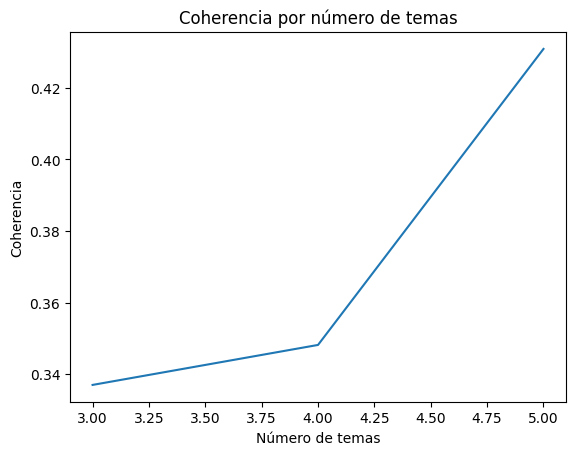
\includegraphics[width=0.5\textwidth]{imagec.png}
    \caption{Coherencia por número de temas.}
    \label{fig:coherencia_temas}
\end{figure}

\subsection{Distribución de los Temas Identificados}

En la Figura \ref{fig:distribucion_temas} se presenta la distribución de los temas en los comentarios analizados. El tema 1 es el más frecuente, con 19 comentarios, seguido de los temas 4 y 5 con 17 y 16 comentarios, respectivamente. 

\begin{figure}[h!]
    \centering
    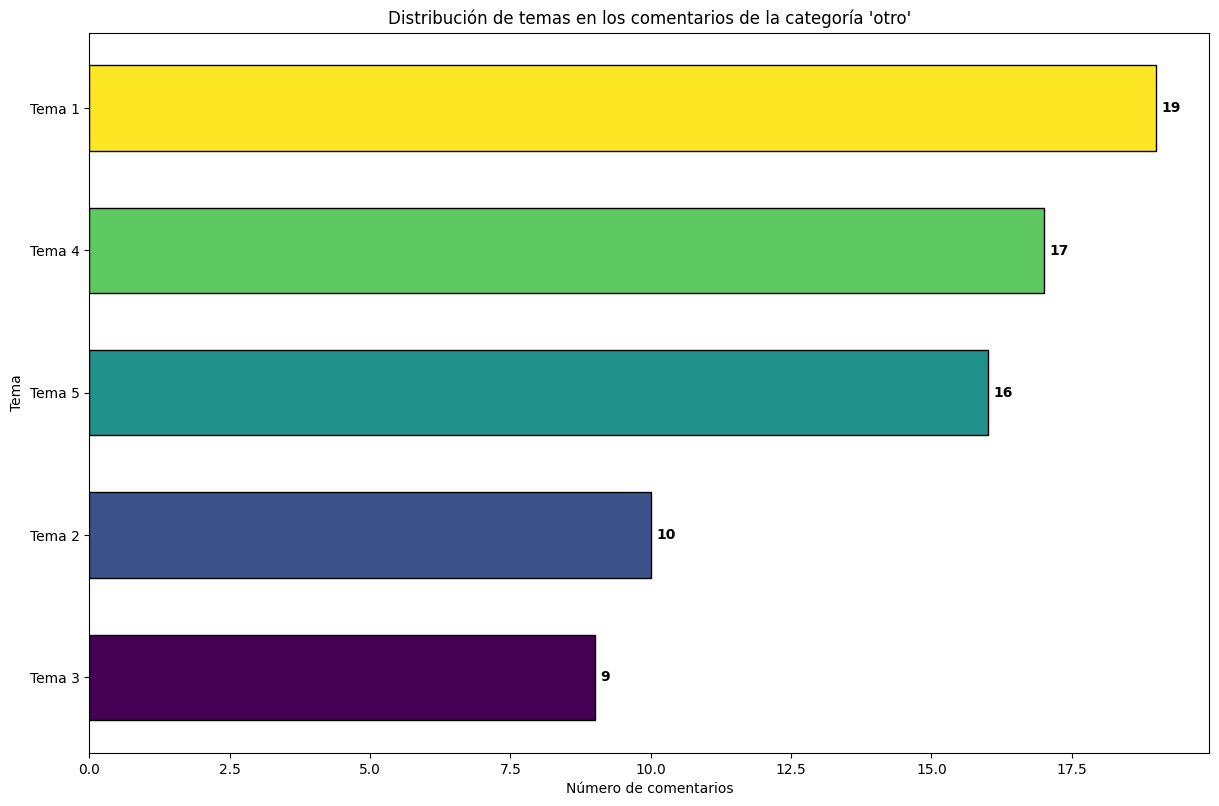
\includegraphics[width=0.8\textwidth]{imaged.png}
    \caption{Distribución de los temas en los comentarios de la categoría ``otro".}
    \label{fig:distribucion_temas}
\end{figure}

\subsection{Interpretación de los Tópicos}

A continuación, se presenta una interpretación de los cinco temas más recurrentes encontrados en los comentarios:

\begin{itemize}
    \item \textbf{Tema 1}: Este tópico refleja una fuerte insatisfacción con el servicio al cliente. Palabras como \textit{``decepción", ``inaceptable", ``respuesta"} indican que los clientes no están recibiendo la asistencia adecuada o en el tiempo esperado.
    
    \item \textbf{Tema 2}: Las quejas en este tópico giran en torno a la actitud y comportamiento de los representantes del banco. Términos como \textit{``grosería", ``relación", ``insatisfactorio"} sugieren que muchos clientes perciben interacciones negativas o poco profesionales.
    
    \item \textbf{Tema 3}: Este tema está relacionado con el tiempo de espera y la rapidez en la atención. Palabras como \textit{``espera", ``minutos", ``rápido"} muestran que la demora en los procesos es una fuente recurrente de quejas entre los clientes.
    
    \item \textbf{Tema 4}: Este tópico se centra en los problemas relacionados con la interacción en sucursales y con el personal del banco. Palabras como \textit{``personal", ``sucursal", ``inquietud"} sugieren que hay deficiencias en el servicio personalizado y en la resolución de dudas o problemas.
    
    \item \textbf{Tema 5}: Este tema hace referencia a problemas técnicos con las aplicaciones bancarias y las transacciones móviles. Términos como \textit{``aplicación", ``transacción", ``fallo"} indican que los usuarios experimentan problemas recurrentes al intentar realizar transacciones a través de la aplicación del banco.
\end{itemize}

En resumen, el modelo de LDA ha permitido identificar áreas clave donde los clientes muestran insatisfacción, tanto en la calidad del servicio al cliente como en problemas técnicos con las plataformas digitales. Estos hallazgos proporcionan una base sólida para diseñar estrategias de mejora enfocadas en reducir las quejas y mejorar la experiencia del cliente.

\subsection{Recomendaciones}

Con base en los resultados obtenidos y el análisis realizado, se proponen las siguientes recomendaciones para BBVA y futuros estudios relacionados con el análisis de comentarios de clientes:

\begin{itemize}

    \item \textbf{Expansión del análisis a otros canales de retroalimentación}: Si bien este estudio se enfocó en comentarios textuales de detractores provenientes de encuestas y redes sociales, sería valioso ampliar el análisis a otros canales de interacción con el cliente, como chats en línea, llamadas al centro de atención y correos electrónicos. Esto permitiría captar una visión más integral de la experiencia del cliente, ya que diferentes canales pueden revelar problemas o inquietudes adicionales.

    \item \textbf{Integración de encuestas de satisfacción instantáneas}: Implementar encuestas de satisfacción en tiempo real, justo después de una interacción con el cliente (por ejemplo, tras el uso de la aplicación móvil o luego de completar una transacción), podría proporcionar datos inmediatos y más precisos sobre la satisfacción del cliente. Esto ayudaría a BBVA a identificar y corregir problemas de forma proactiva.

    \item \textbf{Desarrollo de modelos predictivos basados en NPS}: Se recomienda utilizar los resultados del análisis de los comentarios junto con el Net Promoter Score (NPS) para desarrollar modelos predictivos que permitan anticipar el comportamiento de los clientes. Estos modelos podrían ayudar a predecir la probabilidad de que un cliente se convierta en detractor o promotor, y permitirían tomar medidas preventivas para reducir la tasa de insatisfacción.

    \item \textbf{Exploración de técnicas de análisis más avanzadas}: Aunque el modelo LDA ha sido útil para identificar los temas principales, sería interesante explorar técnicas más avanzadas como modelos basados en \textit{embeddings} (por ejemplo, \textit{BERT} o \textit{Word2Vec}) que capturan mejor el contexto semántico de los comentarios. Estos modelos podrían proporcionar una visión más detallada de las preocupaciones de los clientes y ayudar a mejorar la clasificación de los comentarios.

    \item \textbf{Automatización de la retroalimentación}: Implementar sistemas automatizados que analicen los comentarios de forma continua, proporcionando reportes periódicos a la alta gerencia. Esta automatización permitiría una respuesta más rápida a los problemas emergentes y contribuiría a un ciclo de mejora continua.

    \item \textbf{Futuros estudios académicos y colaboraciones}: Para mejorar la robustez de los modelos desarrollados, sería beneficioso fomentar colaboraciones con instituciones académicas, que podrían explorar enfoques innovadores en la mejora del análisis de sentimiento y la identificación de patrones en grandes volúmenes de datos textuales. Además, futuros estudios podrían enfocarse en comparar la efectividad de diferentes algoritmos de análisis de texto en el contexto bancario.

\end{itemize}

En síntesis, estas recomendaciones buscan ampliar el alcance de las herramientas de análisis desarrolladas y plantean líneas de estudio para perfeccionar la estrategia de atención al cliente en BBVA, con el objetivo de mejorar la satisfacción general y reducir el número de detractores.

\section{Anexos}
Los anexos de este trabajo incluyen el código desarrollado en Google Colab: \url{https://colab.research.google.com/drive/1AVMlirkqufPE-BpA9_ZLStWFVA-XSetJ?usp=sharing} y la Base de datos: \url{https://pub.towardsai.net/bank-complaints-fictional-data-b885cc907b7d}

\section{Referencias}
\begin{thebibliography}{99}
\bibitem{1} Nelson Salgado Reyes, Graciela Elizabeth Trujillo Moreno, «Análisis de sentimientos en datos de redes sociales: aplicación de técnicas de procesamiento de lenguaje natural y machine learning para analizar opiniones y sentimientos en datos de redes sociales,» 2024. URL: \url{https://dspace.itsjapon.edu.ec/xmlui/handle/123456789/4606}.
\bibitem{2} BBVA, «BBVA Colombia, 60 años de historia,» BBVA.com, 2023. URL: \url{https://www.bbva.com/es/co/bbva-colombia-60-anos-historia/}.
\bibitem{3} BBVA, «BBVA Colombia lidera la transformación digital del sector,» BBVA.com, 2023. URL: \url{https://www.bbva.com/es/bbva-colombia-lidera-la-transformacion-digital-del-sector/}.
\bibitem{4} BBVA, «El 2023 fue el año de hacer inversiones récord en Colombia: Mario Pardo, presidente de BBVA en Colombia,» BBVA.com, 2024. URL: \\\url{https://www.bbva.com/es/co/economia-y-finanzas/el-2023-fue-el-ano-de-hacer-inversiones-record-en-colombia-mario-pardo-presidente-de-bbva-en-colombia/}.
\bibitem{5} Hotjar, «Análisis del NPS: 5 formas de entender tu resultado NPS,» Hotjar.com, 2023. URL: \url{https://www.hotjar.com/es/net-promoter-score/analisis/}.
\bibitem{6} Elastic, «¿Qué es el análisis de sentimiento? Una guía completa del análisis de sentimiento,» Elastic.co, 2023. URL: \url{https://www.elastic.co/es/what-is/sentiment-analysis}.
\bibitem{7} Towards AI, «Bank Complaints Fictional Data,» Towards AI, 2023. URL: \url{https://pub.towardsai.net/bank-complaints-fictional-data-b885cc907b7d}.
\bibitem{8} Nazar Anchorena, C., «Extracción de patrones en las reseñas sobre celulares mediante el modelado de temas y el análisis de sentimientos,» Universidad Torcuato Di Tella, 2022. URL: \url{https://repositorio.utdt.edu/bitstream/handle/20.500.13098/11861/MiM_Nazar%20Anchorena_2022.pdf?isAllowed=y&sequence=1}.
\bibitem{9} David M. Blei, Andrew Y. Ng, Michael I. Jordan, «Latent Dirichlet Allocation,» Journal of Machine Learning Research, 3(2003), pp. 993-1022. URL: \url{https://www.jmlr.org/papers/volume3/blei03a/blei03a.pdf}.
\bibitem{10} Florian Rosner, Andreas Hinneburg, Michael Röder, Matthias Nettling, Andreas Both, «Evaluating topic coherence measures,» NIPS 2013 Workshop on Topic Models: Computation, Application, and Evaluation, 2013. URL: \url{https://mimno.infosci.cornell.edu/nips2013ws/nips2013tm_submission_7.pdf}.
\end{thebibliography}

\end{document}

